\chapter{System Modelling and Problem formulation}

The most straightforward way to test the decentralization hypothesis is
to build upon the controller and optimizer introduced in [4]. We will refer
to these controller and optimizer as the Classical Control Stack (CCS).
Instead of forcing the policy to learn everything
from scratch, we can rely on the CCS since can already fly and generate trajectories 
in a centralized fashion. We just need to make the policy learn to mimic,
correct and augment its behavior under loss and reconstruction of some
information. 

The structure of the CCS lends itself
easily to decentralization, hence, we will exploit this property and use
parts of it and its architecture. This will be discussed in detail in
later sections, for now we start by defining the problem, how the
classical control pipeline solves it and what will be our modifications
to decentralize it. The system model and the CCS were mainly developed in[3] and [4].

\section{System Model}

Consider a system of n ≥ 3 non-stopping rigid carriers collaboratively
carrying a rigid payload using cables. The carriers are required to
maintain a strictly positive velocity to avoid stalling. The connection
positions between the cables and the payload are known. Refer to
Figure~\ref{fig:system-model} for a schematic representation of the
considered scenario.

Remark 1: In [3], it is established that a minimum of three non-stopping
carriers are needed to maintain a cable suspended load static while
allowing for each carrier to maintain a loitering positive velocity norm.

Modelling assumptions:

\begin{itemize}
  \item The cables are massless and inextensible
  \item The cables are taut and can only transmit tensile forces
  \item The carriers and the load are rigid bodies
\end{itemize}

Let the inertial world frame $\mathcal{F}_W = \{O_W, (x_W, y_W, z_W)\}$,
with gravity acting along the opposed direction of the $z_W$-axis, and let
the payload’s body-fixed frame $\mathcal{F}_L$ be attached to the
payload’s center of mass (CoM). Let the payload mass be $m_L \in
\mathbb{R}_{>0}$ and inertia matrix $J_L \in \mathbb{R}^{3\times3}$. Let
the $i$-th, $i \in \{1,\dots,n\}$, carrier mass be $m_i \in
\mathbb{R}_{>0}$. The $i$-th carrier is connected to a fixed attachment
point $B_i$ on the payload via a cable of constant length $L_i \in
\mathbb{R}_{>0}$, with unit direction vector $q_i(t) \in \mathbb{S}^2$
pointing from the attachment point to the carrier (representing the cable
direction in the inertial frame).

\begin{figure}[htb]
  \centering
  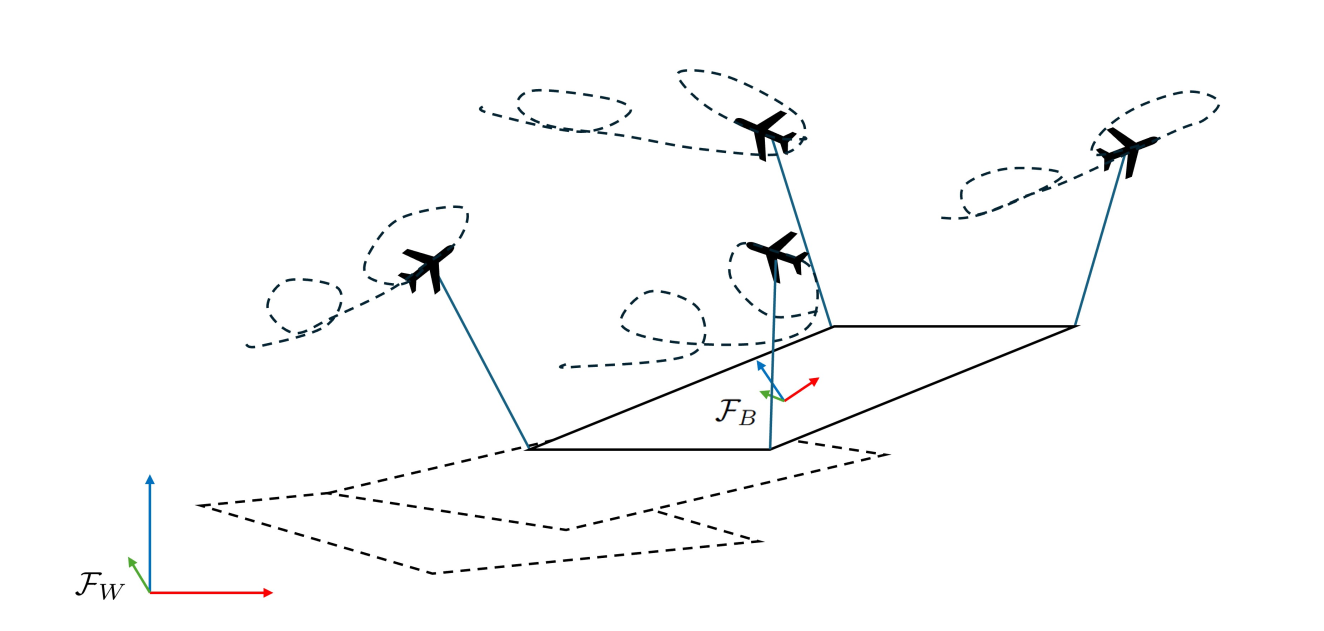
\includegraphics[width=0.85\textwidth]{figures/fig-system-model.png}
  \caption{Schematic representation of $n$ non-stopping fixed-wing
  carriers connected via cables to a rigid payload, showing the inertial
  world frame $\mathcal{F}_W$ and the payload's body-fixed frame
  $\mathcal{F}_B$.}
  \label{fig:system-model}
\end{figure}

We can then calculate the position of the $i$-th carrier $p_{R_i}(t) \in
\mathbb{R}^3$ expressed in $\mathcal{F}_W$ using:

\begin{equation}
  p_{R_i}(t) = p_L(t) + R_L(t)\,{}^{B}b_i + L_i q_i(t)
  \label{eq:carrier-position}
\end{equation}

where $p_L(t) \in \mathbb{R}^3$ and $R_L(t) \in SO(3)$ denote the payload
position and orientation in $\mathcal{F}_W$, and ${}^{B}b_i \in
\mathbb{R}^3$ represent the cable attachment points expressed in
$\mathcal{F}_L$. By differentiating \eqref{eq:carrier-position} we get

\begin{equation}
  \dot{p}_{R_i}(t) = \dot{p}_L(t) + \dot{R}_L(t)\,{}^{B}b_i + L_i \dot{q}_i(t)
  \label{eq:carrier-velocity}
\end{equation}

with $\dot{R}_L(t) = R_L(t) S(\omega_L(t))$ where $\omega_L(t) \in
\mathbb{R}^3$ is the payload angular velocity w.r.t. $\mathcal{F}_W$,
expressed in $\mathcal{F}_L$, and $S(\cdot)$ is the skew-symmetric
operator

Equations \eqref{eq:carrier-position} and \eqref{eq:carrier-velocity}
show that the carriers’ position and velocity are inherently constrained
by the load state and the geometrical configuration of the attachment
point and the cable.

This means that the forces are the real command from whatever control
strategy we design, and determining the desired position and velocity is
a matter of solving the kinematic equations \eqref{eq:carrier-position}
and \eqref{eq:carrier-velocity}. This is also relevant for choosing the
action space of the policy. Instead of trying to output
position/velocity/acceleration set points for the drones, we will output
forces directly since this is the true independent variable that
determine the carriers’ and the payload’s state. In particular, $q_i(t)$
and $\dot{q}_i(t)$ control the carriers’ state. While they can be seen as
the cable direction and its derivative, they also serve as unit vectors
defining the directions of the forces.

\begin{equation}
  f_i(t) = T_i(t) q_i(t)
  \label{eq:cable-force}
\end{equation}

where $T_i(t) \in \mathbb{R}_{\geq 0}$ is the tension in the $i$-th cable
and it generates a force $f_i(t) \in \mathbb{R}^3$ on the payload along
the direction $q_i$.

The payload dynamics follow the Newton–Euler equations:

\begin{align}
  m_L \ddot{p}_L(t) &= -m_L g e_3 + \sum_{i=1}^n f_i(t), \label{eq:newton} \\
  J_L \dot{\omega}_L(t) &= -\omega_L(t) \times J_L \omega_L(t) + \sum_{i=1}^n S({}^{B}b_i)\, R_L(t)^\top f_i(t). \label{eq:euler}
\end{align}

Let $f(t) = [f_1(t)^\top \ \dots \ f_n(t)^\top]^\top \in \mathbb{R}^{3n}$
be the collection of the cable forces. And let $w(t) =
[f_L(t)^\top\ \tau_L(t)^\top]^\top \in \mathbb{R}^6$ representing the
wrench at the load CoM, where $f_L(t) \in \mathbb{R}^3$ and $\tau_L(t) \in
\mathbb{R}^3$ denote the force and the moment components, respectively.
The relation between the these vectors is given by

\begin{equation}
  w(t) = G(R_L(t)) f(t),
  \label{eq:wrench-map}
\end{equation}

where $G(R_L(t)) \in \mathbb{R}^{6 \times 3n}$ is the grasp matrix defined
as

\begin{equation}
  G(R_L(t)) = \begin{bmatrix} I_3 & \cdots & I_3 \\ S({}^{B}b_1) R_L(t)^\top & \cdots & S({}^{B}b_n) R_L(t)^\top \end{bmatrix}.
  \label{eq:grasp-matrix}
\end{equation}

It is easy to see that the first three rows map the forces $f$ to
translational force $f_L(t)$. On the other hand, the last three rows map
them to the moment $\tau_L(t)$ about the payload CoM. We can see that
this map depends on the load orientation $R_L$ and the fixed attachment
points ${}^{B}b_i$ in the body frame.

This formulation enables efficient computation of the cable forces
required to generate a desired load wrench, while providing the basis for
internal force allocation and coordinated control of the carriers.

Indeed, we have that

\begin{equation}
  f(t) = \underbrace{G(R_L(t))^\dagger w(t)}_{=:\, f_g(t)} + \underbrace{N(R_L(t)) \lambda(t)}_{=:\, f_\lambda(t)},
  \label{eq:force-decomposition}
\end{equation}

where $(\cdot)^\dagger$ indicates the right pseudo inverse and
$N(R_L(t))$ is a matrix whose columns identify a basis of the nullspace
of $G(R_L(t))$.

Assuming that the attachment points on the load are well designed, we can
guarantee that $\mathrm{rank}(G(R_L(t))) = 6$. Consequently, dimension of
$\mathrm{null}(G(R_L(t)))$ is $3n - 6$ which is equal to the number of
columns of $N(R_L(t))$ and the number of independent internal forces
component. This number of independent internal force components defines
how many degrees of redundancy are available in the system. This
redundancy allows for internal forces $f_\lambda(t) \in \mathbb{R}^{3n}$
belonging to $\mathrm{null}(G(R_L(t)))$ to redistribute the cable tension
forces without changing the applied wrench on the load and by extension
its motion. Since this work doesn’t go into the design of the classical
control pipeline, the choice of $N(R_L(t))$ to parameterize these
internal forces by a set $\lambda(t)$ of $n$ functions was used as is
from [3].

As a consequence of this architecture, the load trajectory tracking is
cleanly isolated from the carrier trajectory feasibility (i.e.
maintaining the velocity norms of all the carriers above a certain
threshold $\varepsilon > 0$).

\begin{equation}
  \|\dot{p}_{R_i}(t)\| \geq \varepsilon > 0.
  \label{eq:velocity-floor}
\end{equation}

Precisely, the load tracking will be completely achieved by controlling
$f_g(t)$ while, the carrier trajectory feasibility will be done by
controlling the internal forces.

\section{Classical Control Stack (CCS)}

\subsection{Load tracking}

The load tracking is achieved by calculating the desired wrench, the
forces necessary to apply this wrench can then be calculated using the
grasp matrix $G(R_L(t))$ using equation \eqref{eq:wrench-map}. To
calculate the desired wrench, simple PID controllers can be used (one for
the forces and one for the torques). But first the error signal must be
provided to these controllers. The desired load trajectory is
characterized by the desired position, orientation, and corresponding
velocities over time, denoted by $p_{L,d}(t) \in \mathbb{R}^3$,
$R_{L,d}(t) \in SO(3)$, $\dot{p}_{L,d}(t)$, and $\omega_{L,d}(t) \in
\mathbb{R}^3$, respectively. The pose and velocity errors of the load
relative to this desired trajectory are defined as follows:

\begin{align}
  e_p(t) &= p_L(t) - p_{L,d}(t) \label{eq:error-position} \\
  e_R(t) &= \tfrac{1}{2} \left(R_{L,d}(t)^\top R_L(t) - R_L(t)^\top R_{L,d}(t)\right)^\vee \label{eq:error-orientation} \\
  e_v(t) &= \dot{p}_L(t) - \dot{p}_{L,d}(t) \label{eq:error-velocity} \\
  e_\omega(t) &= \omega_{L,d}(t) - \omega_L(t) \label{eq:error-angular-velocity}
\end{align}

Where $(\cdot)^\vee$ is the inverse of the skew-symmetric operator

Given these errors, the desired load wrench $w_d(t) =
[f_{L,d}(t)^\top\ \tau_{L,d}(t)^\top]^\top$ can be calculated using the
PID controllers as follows:

\begin{align}
  f_{L,d}(t) &= m_L g e_3 - K_p e_p(t) - K_v e_v(t) - K_i \int_0^t e_p(\tau)\, d\tau, \label{eq:desired-force} \\
  \tau_{L,d}(t) &= \omega_L(t) \times J_L \omega_L(t) - K_R e_R(t) - K_\omega e_\omega(t) - K_{iR} \int_0^t e_R(\tau)\, d\tau, \label{eq:desired-torque}
\end{align}

with tunable gains $K_p, K_v, K_i, K_R, K_\omega, K_{iR} \in
\mathbb{R}^{3 \times 3}$

\subsection{Carrier Trajectory / Internal Force Calculation: Optimization layer}

By construction, the internal cable force components $f_\lambda(t)$ in
\eqref{eq:force-decomposition} do not have an effect on the wrench
applied to the load CoM. In [4], a method of controlling these forces
online is formulated. An optimization problem is solved at each time step
to keep the carrier velocities above a specified threshold.

While we do not intend to use this optimizer in the solution presented in
this work, its structure is still relevant because we will attempt to
mimic its behavior (we will expand on this point in a later section).
Consequently, it is worth to briefly cover it.

Given $w_d(t)$ based on \eqref{eq:desired-force}-\eqref{eq:desired-torque},
and the corresponding cable forces $f(t) \in \mathbb{R}^{3n}$ generating
such a wrench is:

\begin{equation}
  f(t) = G(t)^\dagger w_d(t) + N(t) \lambda(t),
  \label{eq:optimizer-force}
\end{equation}

where $\lambda(t)$ represents a functional variable to be optimized, and
we use the short hand $G(t) = G(R_L(t))$ and $N(t) = N(R_L(t))$.

The choice of $\lambda(t)$ and design of $N(t)$ was extensively studied
in [3] and [4]. In this work, it is sufficient for us to just take them
as inputs. $\lambda(t)$ is of particular interest, since it will be the
main lever to shape the internal forces of the carriers. It is chosen to
be:

\begin{equation}
  \lambda_i(\xi(t), A(t), t) = A(t) \cos(\xi(t) t + \phi_i)
  \label{eq:lambda-def}
\end{equation}

Where the parameters $\phi_i \in [-\pi, \pi)$, $i = 1, \dots, n$ represent
the constant phase shifts of the carrier (not necessarily distinct but
some have to be).

Whereas the pair $x(t) = (\xi(t), A(t))$ represent the magnitude and the
frequency and are optimized online to enforce a desired lower-bound on
the norm of the carrier velocities as in eq. \eqref{eq:velocity-floor}
(they are shared among the carriers).

Moreover, it can be shown that the force derivative (required to
calculate $\dot{q}_{i,d}(t)$ and hence $\dot{p}_{R_i,d}(t)$) can be
calculated analytically and numerically from the previous equations.

The optimization problem solved online is

\begin{equation}
  x^\star(t) = \operatorname*{arg\,min}_{x(t) \in \mathbb{R}^2} J(x(t)) \quad \text{s.t.} \quad \text{eq. \eqref{eq:velocity-floor}} \ \ \forall i = 1, \dots, n,
  \label{eq:optimization-problem}
\end{equation}

with the objective function

\begin{equation}
\begin{split}
  J(x(t)) = {}& (\xi(t) - \xi(t^-))^2 + (A(t) - A(t^-))^2 \\
  &+ w_{\mathrm{pos}} \|\lambda(x(t)) - \lambda(x(t^-))\|_2^2 + w_{\mathrm{vel}} \|\dot{\lambda}(x(t)) - \dot{\lambda}(x(t^-))\|_2^2.
\end{split}
  \label{eq:objective-function}
\end{equation}

where $t^-$ denotes the previous time instant, and $w_{\mathrm{pos}}$ and
$w_{\mathrm{vel}}$ weighting factors (in this implementation they were
observed to be not helpful therefore set to zero). The cost function is
designed to penalize large instantaneous variations in the cable forces,
thereby reducing abrupt changes in the carriers' trajectories. Solving
the optimization problem yields the optimal coefficients of the internal
force function, $\lambda_i(\xi^*(t), A^*(t), t) \equiv \lambda_i^*(t)$,
for $i = 1, \dots, n$.

In summary, the load state and its reference are used to calculate the
desired wrench $w_d$. Additionally, the load state is also used to
calculate $G(t)$ and $N(t)$. Finally, the optimizer calculates
$\lambda(t)$. They are combined as in eq. \eqref{eq:force-decomposition}
to generate the desired force which is then used in eq.
\eqref{eq:carrier-position} and \eqref{eq:cable-force} to calculate the
desired position. The desired velocity is calculated from the desired
force derivative which can be calculated in a similar albeit more
involved manner. The desired positions and velocities are then passed to
the low level controller of each drone.

\begin{figure}[htb]
  \centering
  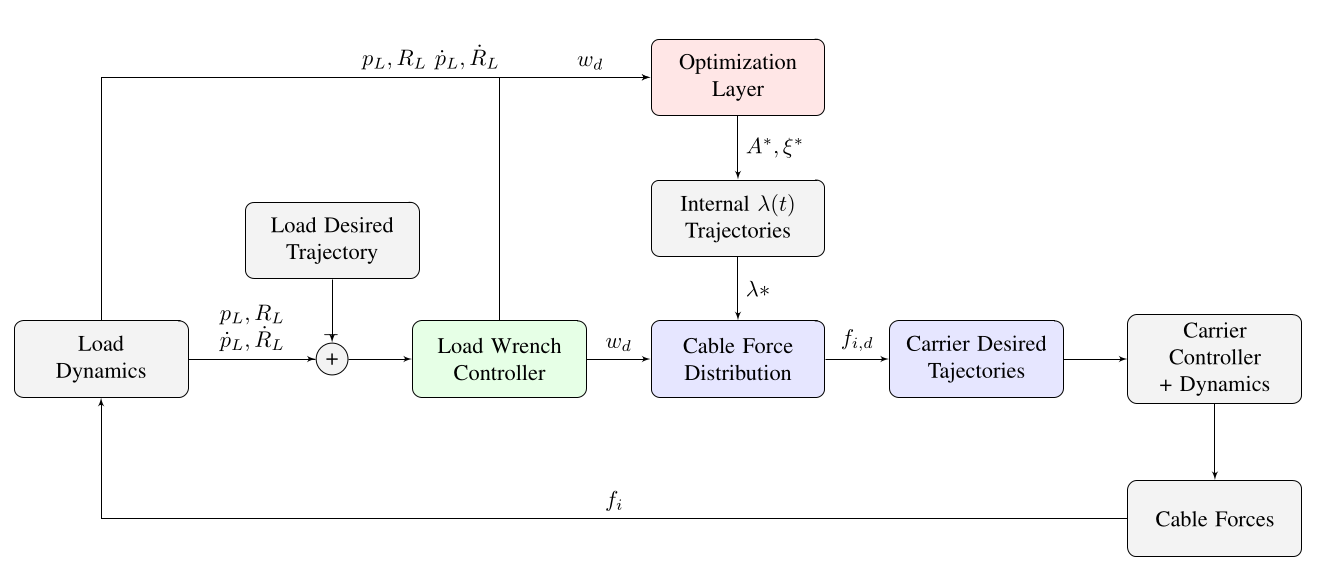
\includegraphics[width=\textwidth]{figures/fig-ccs-pipeline.png}
  \caption{Overall classical control pipeline scheme, including the
  load-wrench controller (green block), the carrier-trajectory generator
  (blue blocks), and the optimization layer (red block).}
  \label{fig:ccs-pipeline}
\end{figure}

\section{Learning-based methods}

This section contains the main problem formulation of the contribution of
this work. To achieve that, we split the work in two phases. Phase one
will mainly target eliminating the optimizer since it takes the bulk of
the computational time per step and therefore it is the biggest obstacle
to onboard deployment. Phase two will focus on modifying the architecture
and using Multi Agent Reinforcement Learning (MARL) to make it fully
decentralized (no communication between the carriers with heterogeneous
asynchronous observations).

\noindent\textbf{Phase One: Imitation Learning(IL)/Behavioral Cloning(BC)}

\noindent Action Space: $\lambda(t) \in \mathbb{R}^n$

\begin{itemize}
  \item Keep wrench controller and nullspace matrix
\end{itemize}

\begin{equation}
  f(t) = f_g(t) + \underline{f_\lambda(t)}
  \label{eq:il-action-force}
\end{equation}

\begin{equation}
  f_\lambda(t) = N(H,t) \cdot \underline{\lambda(t)}
  \label{eq:il-nullspace-force}
\end{equation}

\begin{itemize}
  \item Load tracking guaranteed by construction ($G \cdot N = 0$)
  \item Doesn’t handle desynchronized or heterogeneous observations
\end{itemize}

Since the optimizer was already shown to work well, the proposed solution
in this phase is to distill its behavior using IL. The goal would be to
train a Neural Network (NN) to mimic the output of the optimizer. We face
an interesting choice here, either to train the NN to output $\lambda(t)$
directly or output just $\xi(t)$, $A(t)$ and we can then reconstruct
$\lambda(t)$ using the time $t$ and phase shifts $\phi_i$ using eq.
\eqref{eq:lambda-def}. Outputting $\xi(t)$ and $A(t)$ would be easier
since they are not as dynamic as $\lambda(t)$ and don’t have a periodic
nature. However, in this work we chose to learn $\lambda(t)$ since this
gives the NN control over the internal forces shape. The NN behavior can
then be modified and fine-tuned using Reinforcement Learning (RL) to
achieve certain requirements. A possible extension would be shaping the
reward function to account for fixed-wings dynamics other than the
non-stopping constraint (e.g. minimum turning radius). Outputting
$\xi(t)$ and $A(t)$ would lock us into using eq. \eqref{eq:lambda-def}
with the frequency and amplitude being our only two degrees of freedom.

\noindent\textbf{Phase two:  Residual MARL}

\noindent Action Space: $\delta f \in \mathbb{R}^{3n}$

\begin{itemize}
  \item Keep wrench controller and use the NN that behaviorally clones the optimizer.
  \item Run decentralized
\end{itemize}

\begin{equation}
  f(t) = f_g(t) + f_\lambda(t) + \underline{\delta f(t)}
  \label{eq:residual-action-force}
\end{equation}

\begin{itemize}
  \item Handles desynchronized or heterogeneous observations
  \item Uses the residual force to maintain sensible carrier trajectories and load trajectory tracking
\end{itemize}

The main motivation behind doing phase one first is to ease the
computational burden of phase two.
